\subsection{Développer l'application}
\subsubsection{Démarrer une instance de développement}
\existstill{1.0.0}

La première étape pour contribuer est de réussir à lancer \emph{Floday} dans un environnement contrôlé sur lequel des tests peuvent être exécutés sans crainte.
Une façon de faire va être décrite dans cette section.

Pour fonctionner, on utilisera deux images \emph{VirtualBox} dont l'une sera un clone de la première. La machine virtuelle de base s'appellera \emph{Floday\_Clean} et la copie de travail courante \emph{Floday\_Work}.
Toute la configuration sera à faire sur \emph{Floday\_Clean}, ce qui permettra de réinitiliser \emph{Floday\_Work} si un déploiement se passe mal.

Je présente ici la procédure d'installation de cette architecture sur une Debian 8.0 (Jessie) avec OpenRC comme système d'init.
Il n'y a cependant aucune restriction quant à celle-ci, vous pouvez utiliser le socle que vous voulez, tant que \emph{LXC} y est correctement supporté.
Notez aussi que \emph{riuk}, le jeu de conteneur de test nécessite \emph{OpenRC}.

La création de cette infra reste assez bancale pour le moment, mais elle a le mérite de fonctionner très bien une fois les galères de l'installation passées.
Le jeu en vaut donc la chandelle !
Voici les étapes~:
\begin{itemize}
	\item Installation de \emph{VirtualBox} sur l'hôte.
	\item Création d'un dossier partagé appelé \emph{floday} entre \path{/opt/floday/} sur la VM et le dépôt Git sur l'hôte. Attention, ce partage doit être en lecture et écriture pour pouvoir passer tous les tests unitaires.
	\item Configurer les réseaux \emph{VirtualBox} pour avoir un pont sur \emph{eth0} et un réseau privé hôte sur \emph{eth1}.
	\item Virer \emph{systemd} pour utiliser \emph{Open-RC} à la place~: \url{http://linuxmafia.com/kb/Debian/openrc-conversion.html}.
	\item Installation des additions invitées : \url{htps://virtualboxes.org/doc/installing-guest-additions-on-debian/}.
	\item Création des dossiers \path{/opt/floday}, \path{/var/lib/floday} et \path{/etc/floday}.
	\item Variables d'environnement à ajouter dans \path{/root/.bash}~:\\
{\tt export FLODAY\_CONTAINERS="/opt/floday/src/containers/";\\
export FLODAY\_T="/opt/floday/t/";\\
export FLODAY\_T\_SRC="/opt/floday/src/";}
	\item {\tt{}apt-get install -y --no-install-recommends bridge-utils cgroup-tools\\
		cgroupfs-mount curl apparmor apparmor-utils lxc}
	\item Édition du fichier \emph{/etc/network/interfaces}~:\\
		\begin{lstlisting}
source /etc/network/interfaces.d/*

# The loopback network interface
auto lo
iface lo inet loopback

# The primary network interface
allow-hotplug eth0

iface eth0 inet dhcp
iface eth1 inet dhcp
# This is an autoconfigured IPv6 interface
iface eth0 inet6 auto

auto lxcbr0
iface lxcbr0 inet static
address 10.0.3.1
netmask 255.255.255.0
		\end{lstlisting}
	\item Écrire le fichier \path{/etc.init.d/floday}.
		Il faudra penser à changer \emph{192.168.1.12} par l'ip de votre VM appartenant à l'interface bridgé avec votre routeur allant vers Internet (vous pouvez facilement la récupérer avec la commande \path{ip addr list eth0}.\\
	\begin{lstlisting}
#!/sbin/openrc-run

depend() {
  need cgroupfs-mount
  need vboxadd
  before backup_watcher
}

start() {
  ebegin "Init Floday stuff"
  brctl addbr lxcbr0
  ifup lxcbr0
  dhclient eth1
  mount -t vboxsf floday /opt/floday
  mount -t vboxsf perlvirtlxc /opt/perlvirtlxc
  echo 1 > /proc/sys/net/ipv4/ip_forward
  iptables -t nat -A POSTROUTING -s 10.0.3.0/24 -o eth0 \
    -j SNAT --to-source 192.168.1.12
  eend 0
}
	\end{lstlisting}
	\item \path{rc-update add floday}
	\item {\tt ln -s /opt/floday/lxc-templates/lxc-flodayalpine $\backslash$\\ /usr/share/lxc/templates/}
	\item {\tt ln -s /opt/floday/floday.cfg /etc/floday/floday.cfg}
	\item {\tt ln -s /opt/floday/t/integration/floday.d/runfile.yml /etc/floday/runfile.yml}
	\item Écrire le fichier \path{/etc/lxc/default.conf}~:
		\begin{lstlisting}
lxc.network.type = veth
lxc.network.link = lxcbr0
lxc.network.flags = up
lxc.network.hwaddr = 00:16:3e:xx:xx:xx
		\end{lstlisting}
	\item {\tt cpan Log::Any::Adapter Test::Exception Backticks Moo Config::Tiny File::Slurp YAML::Tiny Template::Alloy Hash::Merge IPC::Run Unix::Syslog}
	\item Ajouter les paramètres \path{apparmor=1 security=apparmor} aux variables \path{GRUB_CMDLINE_LINUX} du fichier \emph{/etc/default/grub}.
	\item {\tt sudo update grub}.
	\item Ajouter la ligne \path{10.0.3.5 test.keh.keh test2.keh.keh} dans le fichier \emph{/etc/hosts} de la machine virtuelle pour pouvoir réussir les tests d'intégrations.
	\item Rebooter la machine virtuelle.
\end{itemize}

Pour valider que la configuration soit correcte, il vous est conseillé de jouer les tests d'intégrations.
S'ils ne passent pas malgré le fait que vous avez scrupuleusement suivi ce guide, vous êtes invités à poster un ticket de type \emph{question} afin que nous puissions enrichir la procédure.

À terme, un script de déploiement automatique sera peut-être fourni.

\subsubsection{Utilisation d'un débogueur}
\existstill{1.2.0}

Nous allons à présent configurer notre espace de travail pour que nous soyons en mesure de déboguer l'exécution de l'application.

\paragraph{Avec \emph{Inteliji IDEA}}

\begin{itemize}
	\item La première étape est bien entendu, d'installer le plugin \emph{Perl} d'\emph{IDEA}.
	\item Il faut ensuite installer le module \emph{CPAN} \path{Devel::Camelcadedb} sur la machine virtuelle précédemment crée.
	\item Dans le \path{.bashrc} de l'utilisateur root de la machine virtuelle, ajouter les variables d'environnement suivantes~:
		\begin{lstlisting}
export PERL5_DEBUG_ROLE='server';
export PERL5_DEBUG_HOST='192.168.56.101';
export PERL5_DEBUG_PORT='8000';
		\end{lstlisting}
	\item Configurer le débogueur \emph{IDEA} comme présenté dans la figure~\ref{dev_dev_dbg_idea}.
		Voici un récapitulatif des valeurs auxquelles il faut penser~:
		\begin{description}
			\item[Remote project root] Il faut renseigner le chemin correspondant à la localité du projet sur la machine virtuelle. Si vous avez suivi à la lettre le paragraphe précédent, la valeur à renseigner devrait être \path{/opt/floday}. Attention, si cette valeur n'est pas la bonne, vous ne pourrez pas utiliser les breakpoints~!
			\item[Connection mode] La valeur conseillée est \path{IDE connects to the perl process}, mais l'inverse fonctionne aussi. Il faudra juste penser à faire les changements adéquats un peu partout.
			\item[Server host] Il s'agit de l'endroit où se situera le processus à débogué. Il faudra renseigner ici l'adresse \emph{IP} de la machine virtuelle. Attention, cette valeur doit être la même que celle présente au niveau de la variable d'environnement \emph{PERL5\_DEBUG\_HOST} que nous avons configuré au point précédent. Normalement, l'ip sera \path{192.168.56.101}.
			\item[Server port] Là aussi, il faut simplement en choisir un d'inoccupé et qu'il soit le même que celui configuré dans la variable \path{PERL5\_DEBUG\_PORT} de la machine virtuelle. Il est conseiller de renseigner la valeur \path{8000}.
		\end{description}
\end{itemize}

Il vous faudra ensuite lancer vos scripts \emph{Perl} avec l'option \path{-d:Camelcadedb}.
Comme par exemple~: \path{perl -d:Camelcadedb floday.pl --host integration}.
L'exécution de l'application sera bloquée jusqu'à ce que vous lancez le débogueur depuis \emph{IDEA} et que celui-ci puisse se connecter au processus.

\begin{figure}
	\centering
	\caption{Configuration du débogueur sur \emph{IDEA}.}
	\label{dev_dev_dbg_idea}
	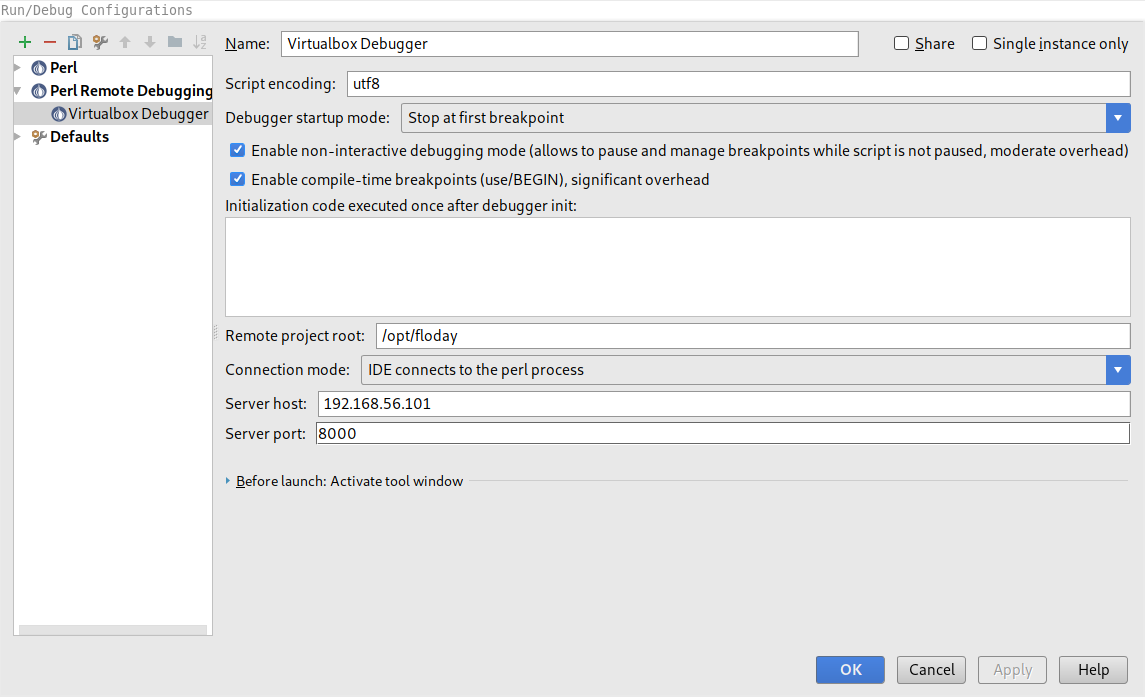
\includegraphics[width=\textwidth]{part/developpement/dev/figs/fig_dbg_idea.png}
\end{figure}

\paragraph{Avec \emph{Vim}}
Il faudra rajouter manuellement la définition des variables d'environnement ci-dessous, dans le ~/.bashrc :

\begin{lstlisting}
export PERL5LIB=/opt/komodo
export PERL5DB="BEGIN {require q(\$PERL5LIB/perl5db.pl)}"
export PERLDB_OPTS="RemotePort=172.17.0.1:9000"
\end{lstlisting}

Actuellement, le débogueur Vim \href{https://github.com/joonty/vdebug}{VDebug} a été testé et fonctionne bien.

Pour installer VDebug, on peut simplement passer via Vundle. Niveau configuration, je vous invite à lire excellente documentation fournie avec le module via la commande Vim d'aide~: \path{:help VDebug}.

Comme le dit la section \emph{VdebugRemoteFilePaths}, il ne faudra pas oublier de faire la correspondance entre le path des fichiers sur votre poste de travail et sur le conteneur. Pour ce faire, rajoutez ceci dans votre \emph{.vimrc}~:

\begin{lstlisting}
let g:vdebug_options = {}
let g:vdebug_options['path_maps'] = {"/opt/floday/":"/path/to/your/floday/repo/"
\end{lstlisting}
